\section*{Methodology}

\subsection*{Neo4j Desktop Setup and Database Import}

To facilitate knowledge graph completion, we utilize Neo4j Desktop for managing and querying the knowledge graph. This subsection provides a step-by-step guide to set up Neo4j Desktop and import a database dump file, as depicted in Figure~\ref{fig:neo4j-setup}. The specific dump used in this midterm report, derived from Hetionet, requires DBMS version $4.3$ to ensure compatibility.

\begin{figure}[ht]
    \centering
    \begin{subfigure}[b]{0.49\textwidth}
        \centering
        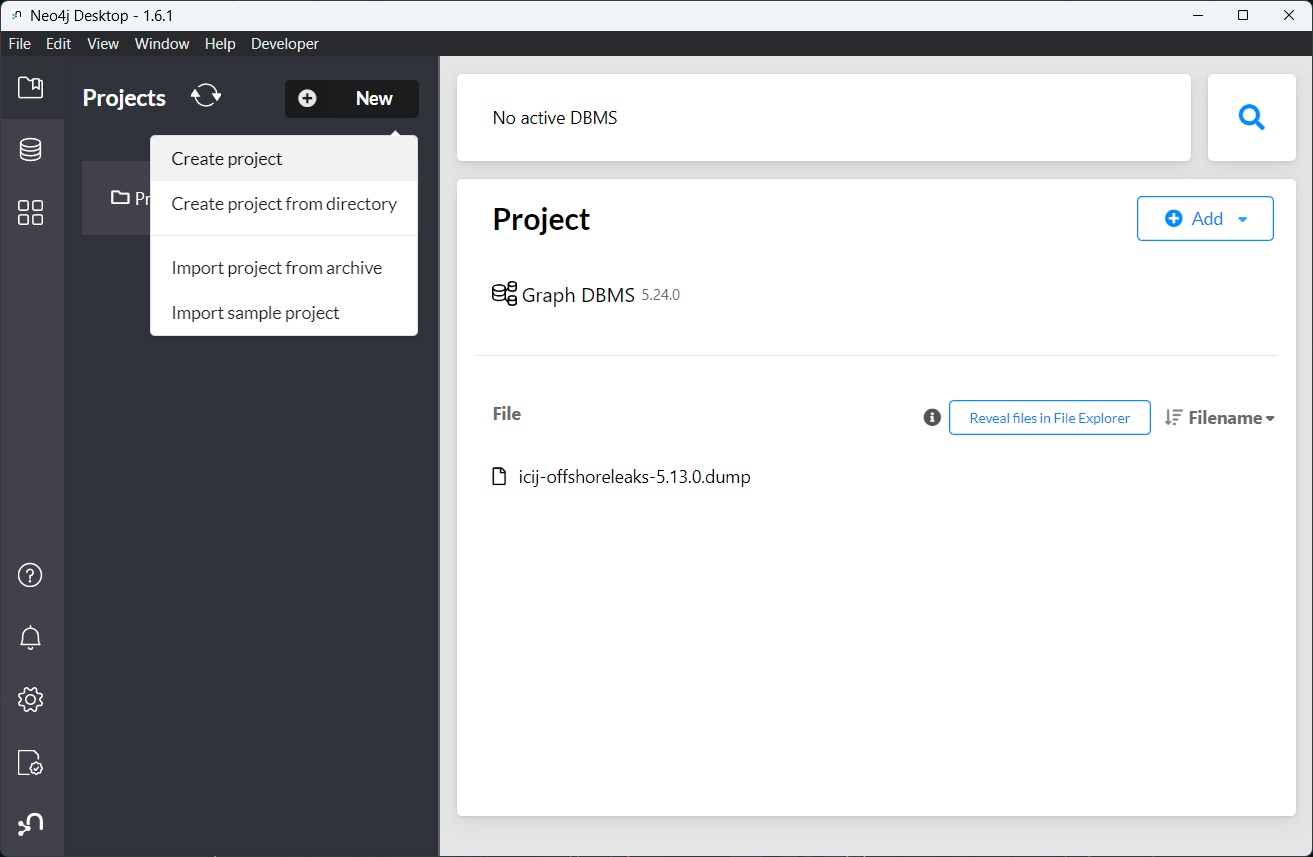
\includegraphics[width=\textwidth]{images/neo4j-setup/1.png}
        \caption{Creating a project.}
    \end{subfigure}
    \hfill
    \begin{subfigure}[b]{0.49\textwidth}
        \centering
        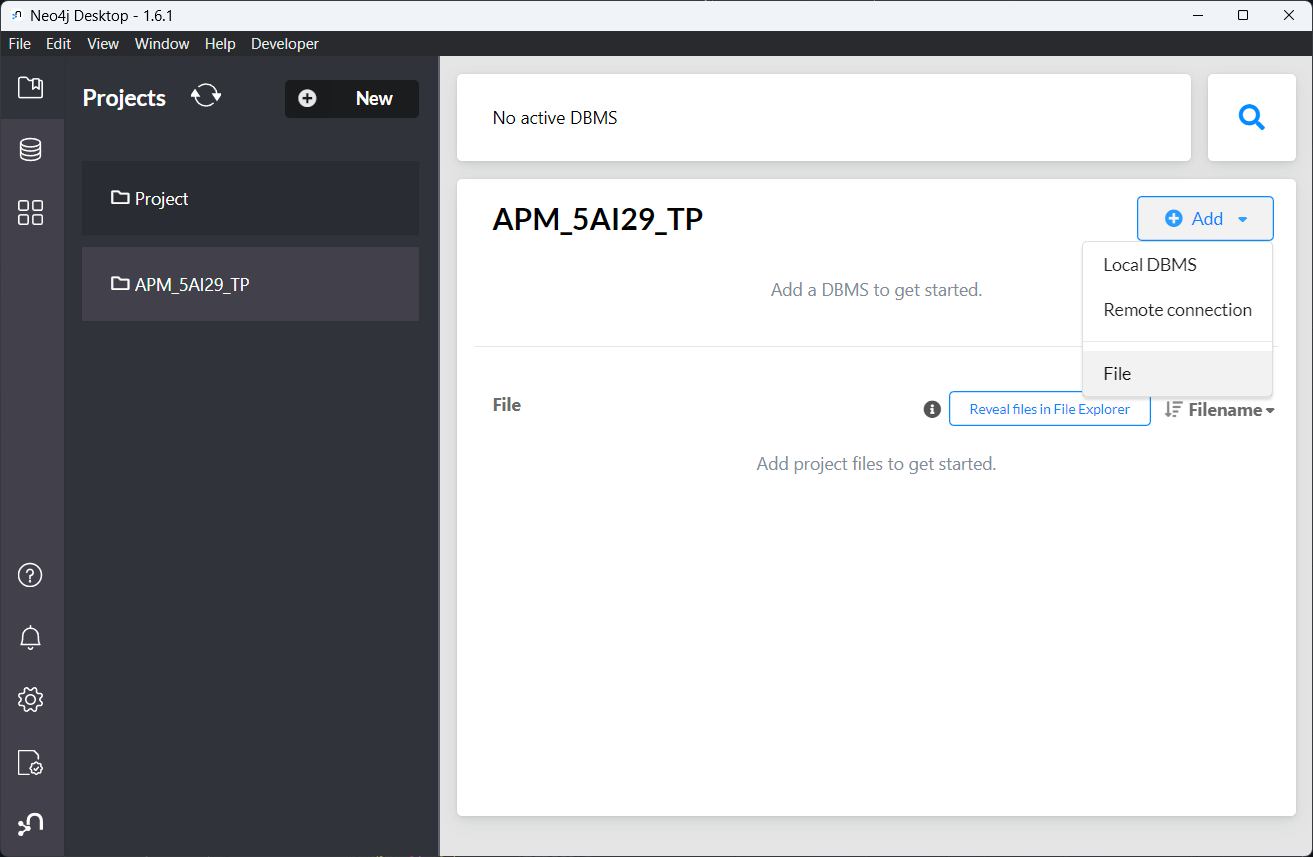
\includegraphics[width=\textwidth]{images/neo4j-setup/2.png}
        \caption{Adding dump file.}
    \end{subfigure}
    \\
    \begin{subfigure}[b]{0.49\textwidth}
        \centering
        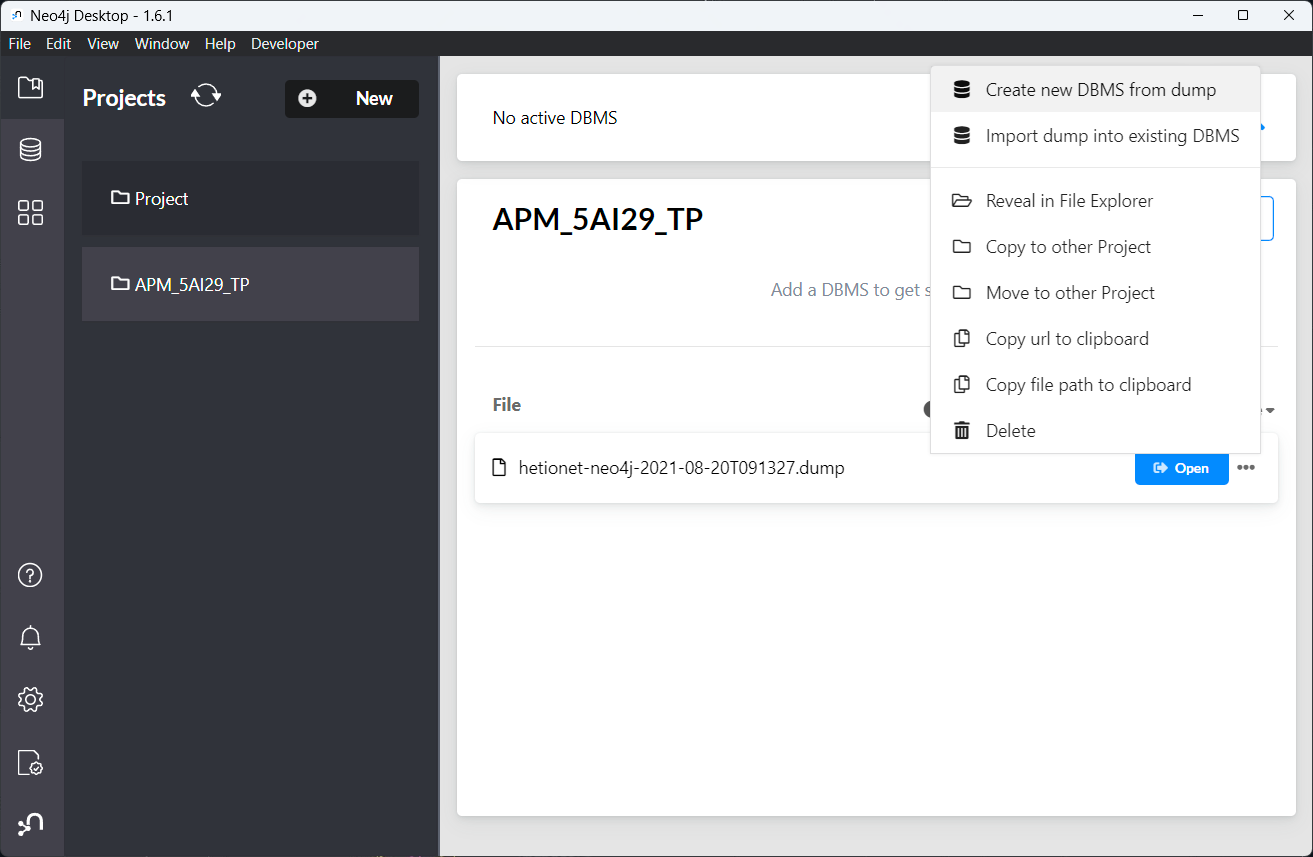
\includegraphics[width=\textwidth]{images/neo4j-setup/3.png}
        \caption{Importing dump to DBMS.}
    \end{subfigure}
    \hfill
    \begin{subfigure}[b]{0.49\textwidth}
        \centering
        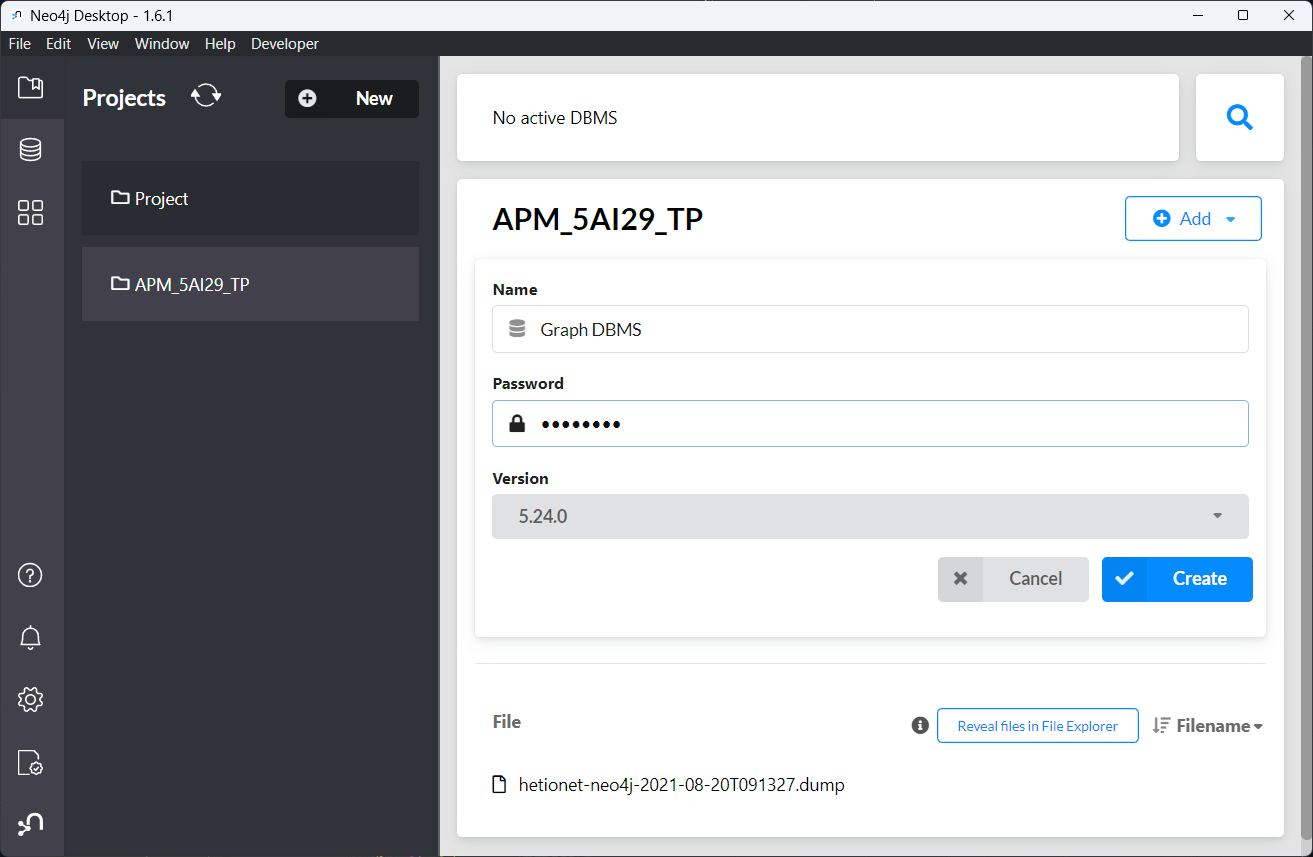
\includegraphics[width=\textwidth]{images/neo4j-setup/4.png}
        \caption{Configuring DBMS.}
    \end{subfigure}
    \\
    \begin{subfigure}[b]{0.49\textwidth}
        \centering
        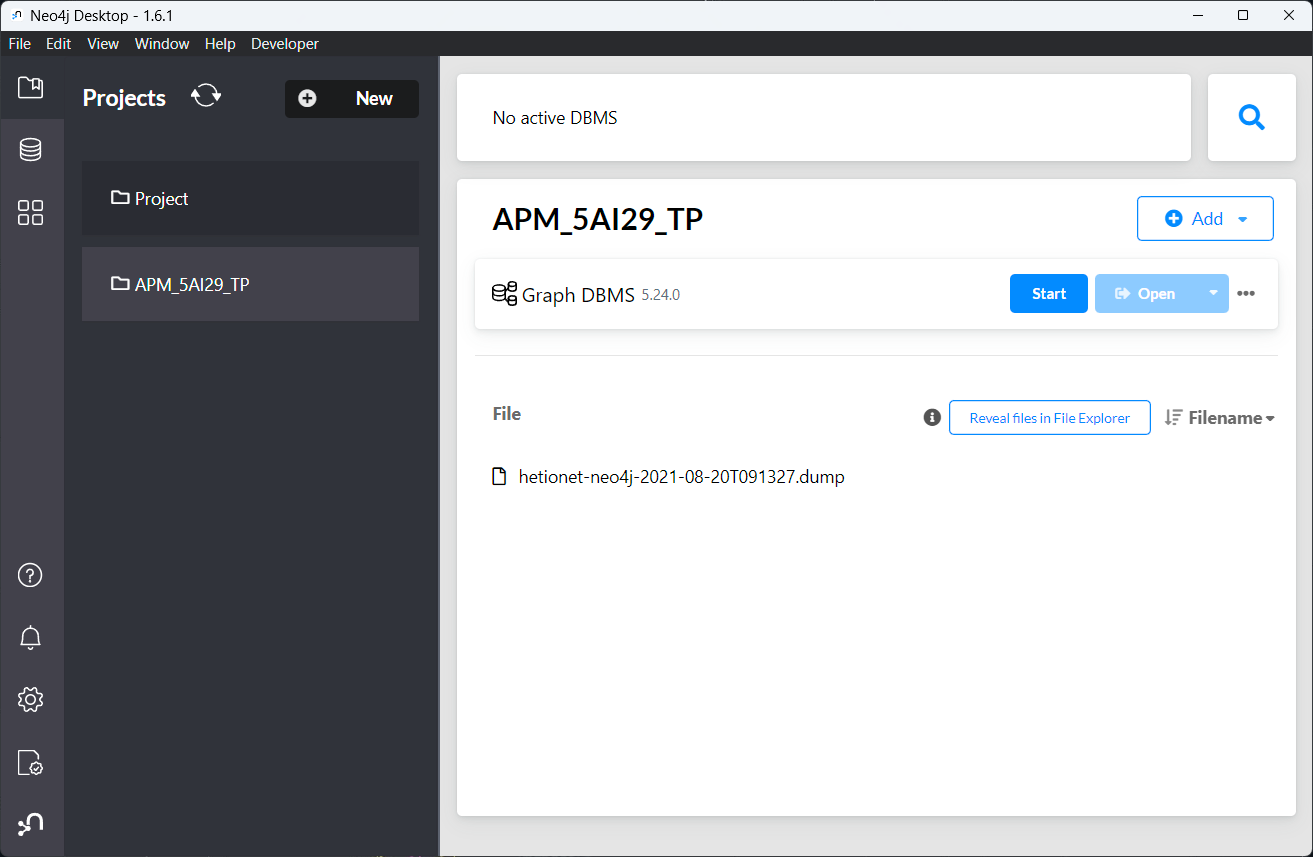
\includegraphics[width=\textwidth]{images/neo4j-setup/5.png}
        \caption{Starting DBMS.}
    \end{subfigure}
    \hfill
    \begin{subfigure}[b]{0.49\textwidth}
        \centering
        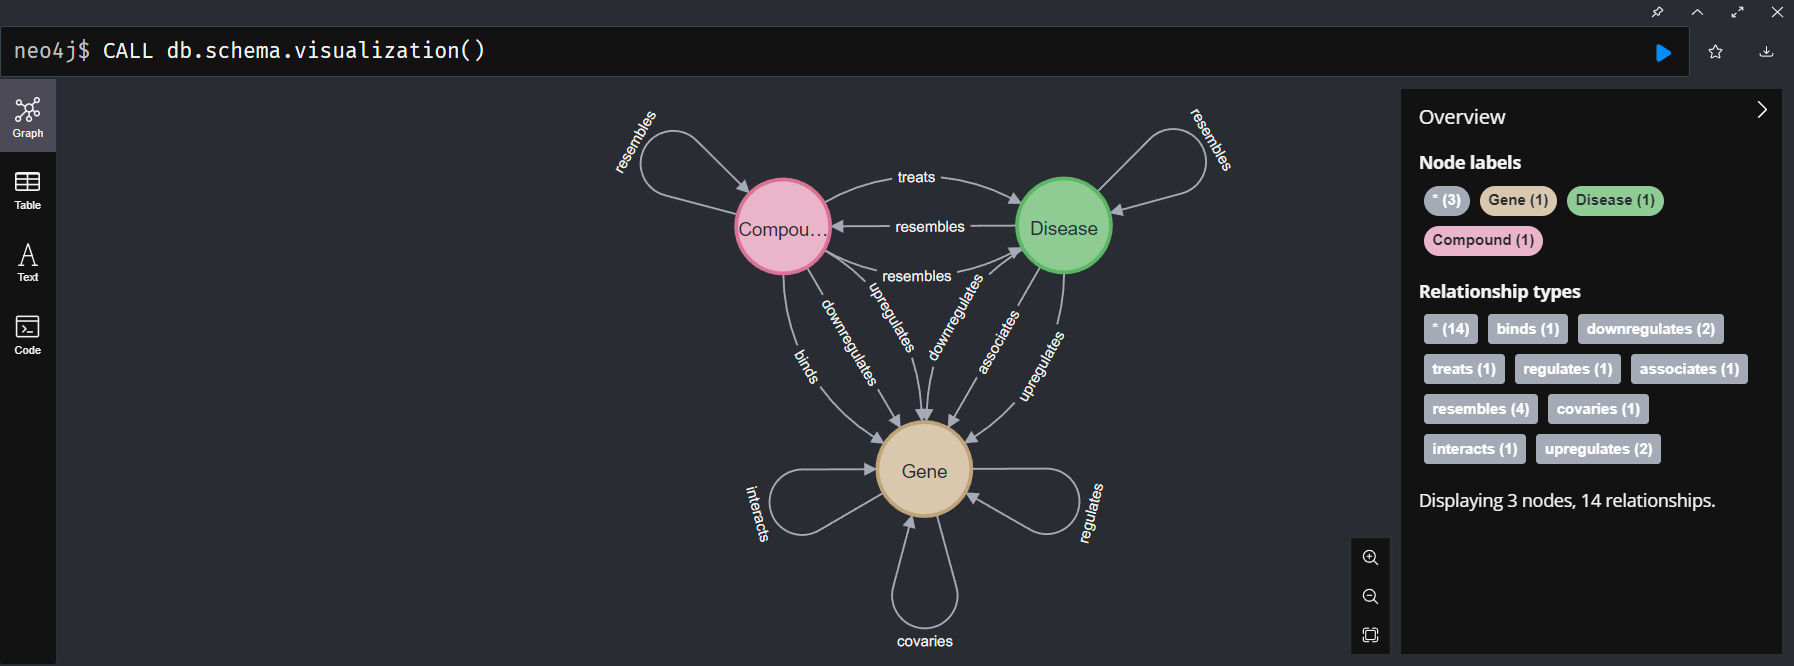
\includegraphics[width=\textwidth]{images/neo4j-setup/7.png}
        \caption{Visualizing schema.}
    \end{subfigure}

    \caption{Steps for Neo4j Desktop Setup.}
    \label{fig:neo4j-setup}
\end{figure}

Upon successful import, the schema can be visualized using the following Neo4j query: \texttt{CALL db.schema.visualization()}. The resulting graph, illustrates key entities and relationships (e.g., \textit{genes, compounds, diseases}) that form the basis for multi-class link prediction and knowledge graph completion in subsequent tasks.
